% Options for packages loaded elsewhere
% Options for packages loaded elsewhere
\PassOptionsToPackage{unicode}{hyperref}
\PassOptionsToPackage{hyphens}{url}
\PassOptionsToPackage{dvipsnames,svgnames,x11names}{xcolor}
%
\documentclass[
  letterpaper,
  DIV=11,
  numbers=noendperiod]{scrartcl}
\usepackage{xcolor}
\usepackage{amsmath,amssymb}
\setcounter{secnumdepth}{5}
\usepackage{iftex}
\ifPDFTeX
  \usepackage[T1]{fontenc}
  \usepackage[utf8]{inputenc}
  \usepackage{textcomp} % provide euro and other symbols
\else % if luatex or xetex
  \usepackage{unicode-math} % this also loads fontspec
  \defaultfontfeatures{Scale=MatchLowercase}
  \defaultfontfeatures[\rmfamily]{Ligatures=TeX,Scale=1}
\fi
\usepackage{lmodern}
\ifPDFTeX\else
  % xetex/luatex font selection
\fi
% Use upquote if available, for straight quotes in verbatim environments
\IfFileExists{upquote.sty}{\usepackage{upquote}}{}
\IfFileExists{microtype.sty}{% use microtype if available
  \usepackage[]{microtype}
  \UseMicrotypeSet[protrusion]{basicmath} % disable protrusion for tt fonts
}{}
\makeatletter
\@ifundefined{KOMAClassName}{% if non-KOMA class
  \IfFileExists{parskip.sty}{%
    \usepackage{parskip}
  }{% else
    \setlength{\parindent}{0pt}
    \setlength{\parskip}{6pt plus 2pt minus 1pt}}
}{% if KOMA class
  \KOMAoptions{parskip=half}}
\makeatother
% Make \paragraph and \subparagraph free-standing
\makeatletter
\ifx\paragraph\undefined\else
  \let\oldparagraph\paragraph
  \renewcommand{\paragraph}{
    \@ifstar
      \xxxParagraphStar
      \xxxParagraphNoStar
  }
  \newcommand{\xxxParagraphStar}[1]{\oldparagraph*{#1}\mbox{}}
  \newcommand{\xxxParagraphNoStar}[1]{\oldparagraph{#1}\mbox{}}
\fi
\ifx\subparagraph\undefined\else
  \let\oldsubparagraph\subparagraph
  \renewcommand{\subparagraph}{
    \@ifstar
      \xxxSubParagraphStar
      \xxxSubParagraphNoStar
  }
  \newcommand{\xxxSubParagraphStar}[1]{\oldsubparagraph*{#1}\mbox{}}
  \newcommand{\xxxSubParagraphNoStar}[1]{\oldsubparagraph{#1}\mbox{}}
\fi
\makeatother


\usepackage{longtable,booktabs,array}
\newcounter{none} % for unnumbered tables
\usepackage{calc} % for calculating minipage widths
% Correct order of tables after \paragraph or \subparagraph
\usepackage{etoolbox}
\makeatletter
\patchcmd\longtable{\par}{\if@noskipsec\mbox{}\fi\par}{}{}
\makeatother
% Allow footnotes in longtable head/foot
\IfFileExists{footnotehyper.sty}{\usepackage{footnotehyper}}{\usepackage{footnote}}
\makesavenoteenv{longtable}
\usepackage{graphicx}
\makeatletter
\newsavebox\pandoc@box
\newcommand*\pandocbounded[1]{% scales image to fit in text height/width
  \sbox\pandoc@box{#1}%
  \Gscale@div\@tempa{\textheight}{\dimexpr\ht\pandoc@box+\dp\pandoc@box\relax}%
  \Gscale@div\@tempb{\linewidth}{\wd\pandoc@box}%
  \ifdim\@tempb\p@<\@tempa\p@\let\@tempa\@tempb\fi% select the smaller of both
  \ifdim\@tempa\p@<\p@\scalebox{\@tempa}{\usebox\pandoc@box}%
  \else\usebox{\pandoc@box}%
  \fi%
}
% Set default figure placement to htbp
\def\fps@figure{htbp}
\makeatother


% definitions for citeproc citations
\NewDocumentCommand\citeproctext{}{}
\NewDocumentCommand\citeproc{mm}{%
  \begingroup\def\citeproctext{#2}\cite{#1}\endgroup}
\makeatletter
 % allow citations to break across lines
 \let\@cite@ofmt\@firstofone
 % avoid brackets around text for \cite:
 \def\@biblabel#1{}
 \def\@cite#1#2{{#1\if@tempswa , #2\fi}}
\makeatother
\newlength{\cslhangindent}
\setlength{\cslhangindent}{1.5em}
\newlength{\csllabelwidth}
\setlength{\csllabelwidth}{3em}
\newenvironment{CSLReferences}[2] % #1 hanging-indent, #2 entry-spacing
 {\begin{list}{}{%
  \setlength{\itemindent}{0pt}
  \setlength{\leftmargin}{0pt}
  \setlength{\parsep}{0pt}
  % turn on hanging indent if param 1 is 1
  \ifodd #1
   \setlength{\leftmargin}{\cslhangindent}
   \setlength{\itemindent}{-1\cslhangindent}
  \fi
  % set entry spacing
  \setlength{\itemsep}{#2\baselineskip}}}
 {\end{list}}
\usepackage{calc}
\newcommand{\CSLBlock}[1]{\hfill\break\parbox[t]{\linewidth}{\strut\ignorespaces#1\strut}}
\newcommand{\CSLLeftMargin}[1]{\parbox[t]{\csllabelwidth}{\strut#1\strut}}
\newcommand{\CSLRightInline}[1]{\parbox[t]{\linewidth - \csllabelwidth}{\strut#1\strut}}
\newcommand{\CSLIndent}[1]{\hspace{\cslhangindent}#1}



\setlength{\emergencystretch}{3em} % prevent overfull lines

\providecommand{\tightlist}{%
  \setlength{\itemsep}{0pt}\setlength{\parskip}{0pt}}



 


\KOMAoption{captions}{tableheading}
\makeatletter
\@ifpackageloaded{caption}{}{\usepackage{caption}}
\AtBeginDocument{%
\ifdefined\contentsname
  \renewcommand*\contentsname{Table of contents}
\else
  \newcommand\contentsname{Table of contents}
\fi
\ifdefined\listfigurename
  \renewcommand*\listfigurename{List of Figures}
\else
  \newcommand\listfigurename{List of Figures}
\fi
\ifdefined\listtablename
  \renewcommand*\listtablename{List of Tables}
\else
  \newcommand\listtablename{List of Tables}
\fi
\ifdefined\figurename
  \renewcommand*\figurename{Figure}
\else
  \newcommand\figurename{Figure}
\fi
\ifdefined\tablename
  \renewcommand*\tablename{Table}
\else
  \newcommand\tablename{Table}
\fi
}
\@ifpackageloaded{float}{}{\usepackage{float}}
\floatstyle{ruled}
\@ifundefined{c@chapter}{\newfloat{codelisting}{h}{lop}}{\newfloat{codelisting}{h}{lop}[chapter]}
\floatname{codelisting}{Listing}
\newcommand*\listoflistings{\listof{codelisting}{List of Listings}}
\makeatother
\makeatletter
\makeatother
\makeatletter
\@ifpackageloaded{caption}{}{\usepackage{caption}}
\@ifpackageloaded{subcaption}{}{\usepackage{subcaption}}
\makeatother
\usepackage{bookmark}
\IfFileExists{xurl.sty}{\usepackage{xurl}}{} % add URL line breaks if available
\urlstyle{same}
\hypersetup{
  pdftitle={The Relationship Between Secondary Education and Nobel Laureates Across Countries},
  pdfauthor={Marlon Trejo},
  colorlinks=true,
  linkcolor={blue},
  filecolor={Maroon},
  citecolor={Blue},
  urlcolor={Blue},
  pdfcreator={LaTeX via pandoc}}


\title{The Relationship Between Secondary Education and Nobel Laureates
Across Countries}
\author{Marlon Trejo}
\date{September 24, 2026}
\begin{document}
\maketitle
\begin{abstract}
We consider whether a country's percentage of the population with at
least some secondary schooling has any association on the number of
nobel laureates that country's had. The regression line shows a slight
upward trend, indicating that, on average, there is a positive
correlation.
\end{abstract}


\section{Introduction}\label{introduction}

Nobel Prizes are awarded in accordance with the principle of ``for the
greatest benefit to humankind''. The six categories are physics,
chemistry, medicine, literature, peace, and economic science. This
analysis was done to determine whether there was a linear relationship
between the percentage of the population with at least some secondary
education in that country, and the number of Nobel laureates in that
country.

The primary motivation is to inspire further research into what aspects
of a country's education system causes high scientific/civil
achievement. This paper is meant to see if education level and Nobel
prizes won per country are correlated. If they aren't, that would
indicate that there's other elements involved (such as talent or
individual strengths) that produces Nobel laureates.

A regression line was fitted, and a slope of .529 was found. A p-test
can't be conducted due to non-constant variance of the errors.

Section~\ref{sec-data} introduces the data used in this analysis.
Section~\ref{sec-methods} describes the statistical model.
Section~\ref{sec-results} presents the results of the analysis, and
Section~\ref{sec-discussion} discusses the findings.

\section{Data}\label{sec-data}

The predictor variable data comes from the official Human Development
Report from the United Nations from 2016 (United Nations Development
Programme 2016). The outcome variable comes from the official Wikipedia
list of Nobel Laureates per Country (Wikipedia contributors 2026). The
outcome variable is the number of Nobel Prize winners from a certain
country. The predictor variable is a percentage, and it corresponds to
the population in that country with at least some secondary education.
This comes from surveys given to people aged 25 or older. Since there
were some countries in the Nobel Prize data but missing in the data set,
those countries were erased, instead of getting the data from an
additional data source (to keep variables consistent). There are obvious
limitations in using surveys-people could lie, or data could be
incomplete.

\section{Methods}\label{sec-methods}

I adopted the simple linear regression model

\[
Y_i = \beta_0 + \beta_1 X_i + \varepsilon_i,
\]

where \(Y_i\) represents the response variable (Number of Nobel Prize
Winners), and \(X_i\) represents the predictor variable (Percent of
Population with at Least Some Secondary Education).

In this model, \(\beta_0\) doesn't mean anything, since it represents
the expected number of Nobel prize winners from a country with no
percent of the population having some secondary education. \(\beta_1\)
represents the expected change in the number of Nobel Prize winners
associated with an increase of one percentage point of the population
having some secondary education. \(\varepsilon_i\) represents elements
that cause the count to differ from the expected value (errors).

I implemented this analysis using the R programming language (R Core
Team, n.d.). Specifically, I used the lm() function in R.

The assumptions of this model include normally distributed and errors,
which we will show to be true later. Potential weaknesses of this
approach might be that the variance doesn't appear to be constant-the
higher the percentage of individuals with at least some secondary
education, the more spread out the number of Nobel Prize winners. Also,
the United States is an obvious outlier.

\section{Results}\label{sec-results}

The estimated regression model is

\[
\widehat{Y}
=
-20.803
+
0.529X.
\]

The estimated slope parameter is \(b_1 =\) 0.529.

In other words, for each additional increase in the percent of the
population with at least some secondary education, the number of Nobel
prize winners in that country changes by approximately 0.529 winners, on
average.

The estimated intercept is -20.803.

We will do no confidence intervals or hypothesis testing, since they
would not be reliable due to the non-constant variance shown by the
residuals.

Figure~\ref{fig-suicide-residual} shows the residuals from the fitted
regression model. The points seem to have a funnel shape near the right,
indicating non equal variance. The data does seem to be normally
distributed, as shown in Figure 3 below.

\begin{figure}

\centering{

\pandocbounded{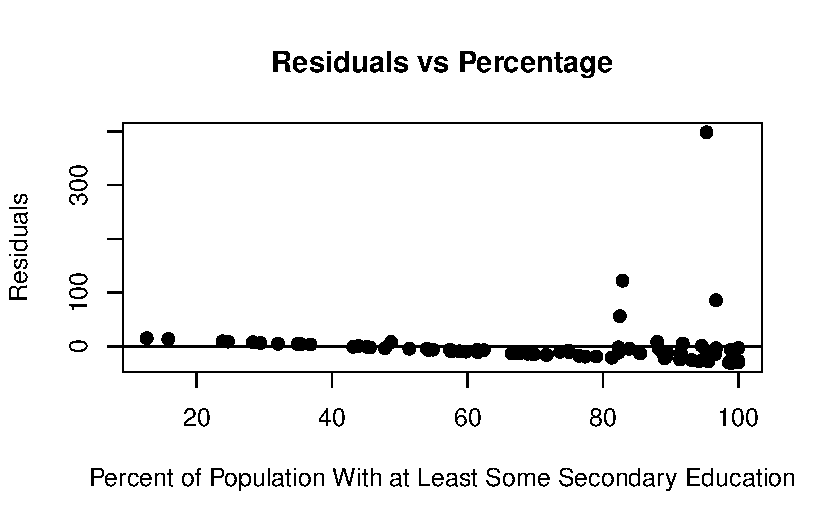
\includegraphics[keepaspectratio]{project_files/figure-pdf/fig-suicide-residual-1.pdf}}

}

\caption{\label{fig-suicide-residual}Residuals from the simple linear
regression model plotted}

\end{figure}%

\begin{figure}

\centering{

\pandocbounded{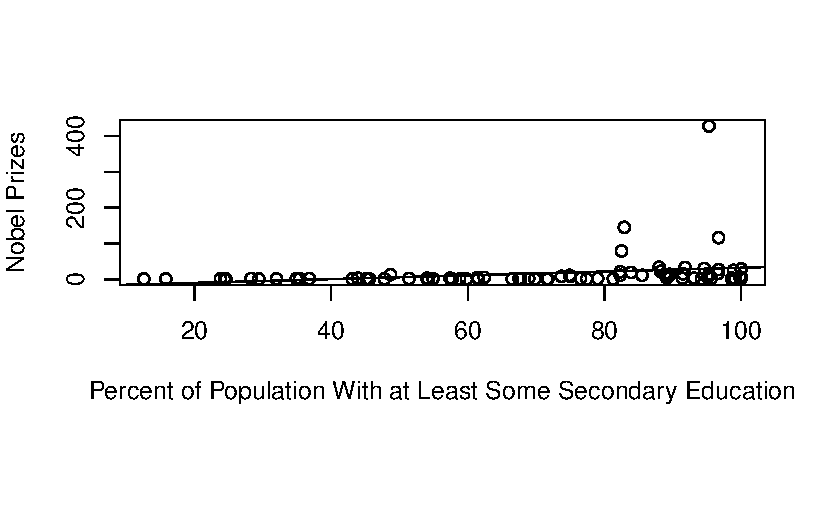
\includegraphics[keepaspectratio]{project_files/figure-pdf/fig-suicide-scatter-1.pdf}}

}

\caption{\label{fig-suicide-scatter}Percent of population with some
secondary education vs.~Nobel Prize winners in that country with fitted
linear regression line.}

\end{figure}%

\begin{figure}[H]

{\centering \pandocbounded{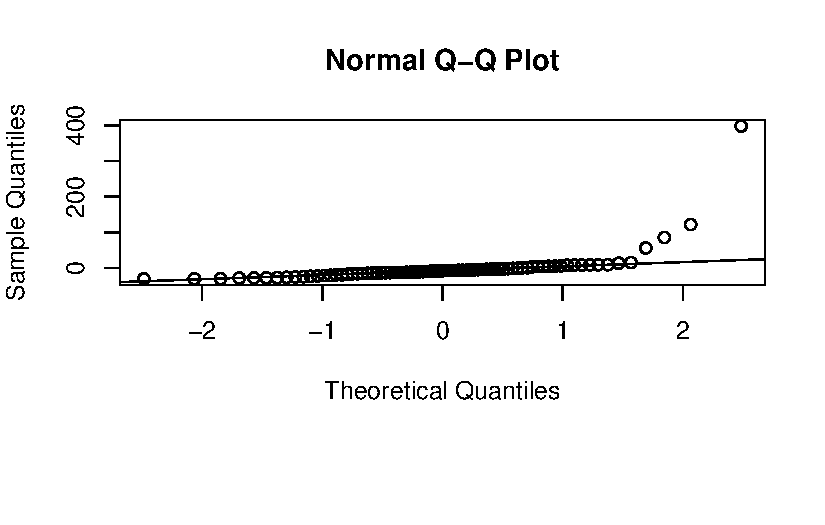
\includegraphics[keepaspectratio]{project_files/figure-pdf/Q-1.pdf}}

}

\caption{QQ Norm Plot.}

\end{figure}%

\section{Discussion}\label{sec-discussion}

This paper attempted to see if there was a linear relationship between
Nobel prize winners per country and the percentage of people with at
least some secondary education in that country. Based on our methods
used, there seems to be a positive linear relationship. There is a
slight upward slope, but a p-test can't be done due to non-constant
variance of the errors. There are some weaknesses in this study,
including the variance of the errors and the fact that the surveys done
probably aren't 100\% accurate. Future work might be better handled by a
more accurate predictor variable and more data.

\protect\phantomsection\label{refs}
\begin{CSLReferences}{1}{1}
\bibitem[\citeproctext]{ref-R_language}
R Core Team. n.d. \emph{R: A Language and Environment for Statistical
Computing}. R Foundation for Statistical Computing.
\url{https://www.R-project.org/}.

\bibitem[\citeproctext]{ref-undp2016}
United Nations Development Programme. 2016. \emph{Human Development
Report 2016: Human Development for Everyone}. United Nations Development
Programme.
\url{https://hdr.undp.org/sites/default/files/hdr_2016_statistical_annex.pdf}.

\bibitem[\citeproctext]{ref-wikipedia_nobel_country}
Wikipedia contributors. 2026. \emph{List of Nobel Laureates by Country}.
Wikipedia.
\url{https://en.wikipedia.org/wiki/List_of_Nobel_laureates_by_country}.

\end{CSLReferences}




\end{document}
